
% DO NOT CHANGE THIS FILE.

% This file contains all the formatting information required
% to make your document fit the necessary style requirements.
% Any changes you make to this file will be over-written at
% the time of submission. If for any reason you feel it is
% necessary to make changes to this, such as a missing package,
% please contact the editors of North East Indian Linguistics
% to discuss the suggested changes.

% DO NOT MAKE ANY CHANGES WITHOUT APPROVAL FROM THE EDITORS.

\documentclass[12pt]{article}

% margins, paper size
\usepackage{geometry} 
\geometry{
	a4paper,
	bottom=2.5cm,
	left=2.5cm,
	right=2.5cm,
	top=2.5cm,
}

% fonts
\usepackage{fontspec}
\newfontfamily\tgtermes{TeX Gyre Termes}
\setmainfont{Times New Roman}[
	ItalicFont={Times New Roman Italic},
	BoldFont={Times New Roman Bold}
]
\newfontfamily\tgtermes{TeX Gyre Termes} % small caps fallback
\makeatletter
  \begingroup
    \tgtermes
    \DeclareFontShape{\f@encoding}{\rmdefault}{m}{sc}{%
      <-> ssub * \f@family/m/sc}{}
    \DeclareFontShape{\f@encoding}{\rmdefault}{bx}{sc}{%
      <-> ssub * \f@family/bx/sc}{}
  \endgroup
\makeatother
\newfontfamily\oblique{Times New Roman Italic}

% bold captions at 10pt
\usepackage[small,font=bf,hang,labelsep=endash]{caption}

% font sizes
\makeatletter
\renewcommand\large{\@setfontsize\large{13pt}{15pt}}
\renewcommand\normalsize{\@setfontsize\normalsize{12pt}{14pt}}
\renewcommand\tiny{\@setfontsize\tiny{8pt}{10pt}}
\renewcommand\scriptsize{\@setfontsize\scriptsize{9pt}{11pt}}
\renewcommand\small{\@setfontsize\small{10pt}{12pt}}
\makeatother

% section title fonts and sizes
\usepackage[compact]{titlesec}
\titleformat{\section}
  {\normalfont\fontsize{12}{12}\bfseries}{\thesection.}{.5em}{}
\titlespacing{\section}{0em}{1.25em}{1em}

% enable footnotes
\usepackage{footnote}

% abstract block visuals
\usepackage{xcolor,colortbl}
\usepackage{makecell}
\usepackage{array}
\newcolumntype{?}{!{\vrule width 1pt}}

% images, used for imported figures &c
\usepackage{graphicx}

% glossing
\usepackage{linguex}
\usepackage{cgloss}
\renewcommand*{\eachwordone}{\oblique}

% tables
\usepackage{booktabs}

% redefine abstract
%\renewcommand{\abstract}[1] {xyz #1}
\renewenvironment{abstract}[1] {
	\begin{table}[h]
	\begin{tabular}{?p{1.75cm}p{13,5cm}?}
	\Xhline{1pt}
	\rowcolor[HTML]{FAD4B6}
	\textbf{\scriptsize Abstract} & \scriptsize\textit{#1} \\
	\tiny{Citation} & \tiny{XXXX. \the\year. XXXXXXXX. North East Indian Linguistics (NEIL), 8. Canberra, Australian National University: Asia-Pacific Linguistics Open Access. issn: xxxx. doi: xxxxx.} \\
	\tiny{Volume Editors} & \tiny{Linda Konnerth, Stephen Morey, Amos Teo} \\
	\tiny{Copyright} & \tiny{© \the\year, the author(s), release under Creative Commons Attribution license} \\
	\tiny{URL} & \tiny{xxxxxxxx} \\ \Xhline{1pt} 
	\end{tabular}
	\end{table}
	\vspace{1em}
}

%\renewenvironment{quote}[1] {
%	\vspace{1em}
%	\small #1
%	\vspace{1em}
%}

\renewenvironment{quote}{
	\small\begin{quotation}
}{
	\end{quotation}
}

% redefine /maketitle
\makeatletter
\def\@maketitle{
  \newpage
  \begin{center}%
  \let \footnote \thanks
    {\large \@title \par}
    \vskip 1em%
    {\oblique
      \begin{tabular}[t]{c}
        \@author
      \end{tabular}\par}
%    \vskip 1em
%    {\small \@date}
  \end{center}
  \par
  \vskip 1em}
\makeatother

% bibliography
\usepackage[
    backend=biber,
    style=authoryear-icomp,
    sortlocale=en_US,
    natbib=true,
    url=false, 
    doi=true,
    eprint=false
]{biblatex}
\addbibresource{references.bib}

% bibliography patching
\usepackage{xpatch}

% temporary lorem ipsum generator
\usepackage{lipsum}

\begin{document}


% Do not change anything above this line

\title{LaTeX Template for Publication in North East Indian Linguistics\footnote{Acknowledgements appear here.}}

\author{Kellen Parker van Dam\\La Trobe University}

\maketitle

\abstract{Quisque ullamcorper placerat ipsum. Cras nibh. Morbi vel justo vitae lacus tincidunt ultrices. Lorem ipsum dolor sit amet, consectetuer adipiscing elit. In hac habitasse platea dictumst. Integer tempus convallis augue. Etiam facilisis. Nunc elementum fermentum wisi. Aenean placerat. Ut imperdiet, enim sed gravida sollicitudin, felis odio placerat quam, ac pulvinar elit purus eget enim. Nunc vitae tortor.}

\section{Write the first heading here}

\lipsum[1]

\begin{quote}
	This is a block quote, with an included citation \autocite{morey2018verbstemalternation}. In order to preserve formatting, be sure to use the \texttt{quote} environment for blockquotes and not \texttt{quotation}.
\end{quote}

\lipsum[5]

\section{Tables \& Figures}

\lipsum[6]

Tables should be centred on the page, with the \texttt{\textbackslash caption\{\}} at the bottom.

\begin{table}[htpb!]
	\centering
	\begin{tabular}{@{}lllll@{}}
	\toprule
	gloss & Needham & Marrison & Das Gupta & modern \\ \midrule
	iron & yân & yan & -- & ʒan \\
	plate &  & -- & -- & pan \\
	cow & mân & -- & man & man \\
	bracelet & sân & san & -- & san \\
	bread & -- & -- & -- & βan \\ \bottomrule
	\end{tabular}
	\caption{The *an rhyme in Muishaung}
	\label{tab:an}
\end{table}

Table \ref{tab:an} is using the \texttt{booktabs} style. This may need to be changed since it doesn't currently match the previous Word template design.

Captions and centring  of figures are handled the same way:

\begin{figure}[htpb!]
  \centering
    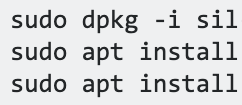
\includegraphics[width=0.25\textwidth]{fig}
  \caption{A simple figure}
\end{figure}

\section{Glossing}

Glossing is handled with the \texttt{linguex} and \texttt{cgloss} packages. Abbreviations should be lowercase and contained in a \texttt{\textbackslash textsc\{\}} tag for small capital letters. The following is from van Dam (\citeyear{vandam2019syntax})

\exg.   kaʔ\textsubscript{4} ko\textsubscript{2} nɤ\textsubscript{2} tə\textsubscript{0}-no\textsubscript{1} ʃɯu\textsubscript{1}\\
		down towards {\textsc{prep}} {\textsc{caus}}-extend.horiz {\textsc{imp}}\\~\\
		`point [something] downwards'

\section{Conclusion}

\lipsum[3]

\section*{Abbreviations}

\vspace{-1em} % for tables immediately following section titles
\begin{table}[htpb!]
    \begin{tabular}{ll}
    \textsc{caus} & Causative prefix \\
    \textsc{imp} & Imperative marker \\
    \textsc{prep} & Preposition
	\end{tabular}
\end{table}

% Do not change anything below this line


% DO NOT CHANGE THIS FILE.

% This file contains all the formatting information required
% to make your document fit the necessary style requirements.
% Any changes you make to this file will be over-written at
% the time of submission. If for any reason you feel it is
% necessary to make changes to this, such as a missing package,
% please contact the editors of North East Indian Linguistics
% to discuss the suggested changes.

% DO NOT MAKE ANY CHANGES WITHOUT APPROVAL FROM THE EDITORS.

\xpatchbibmacro{date+extrayear}{
  \printtext[parens]%
}{
  \setunit{\addperiod\space}
  \printtext
}{}{}

\printbibliography

\end{document}